%%%%%%%%%%%%%%%%%%%%%%%%%%%%%%%%%%%%%%%%%
% Merged Hanami Paper
% Using format from introduction.tex
% Incorporating content from overview.tex and system_architecture.tex
% Updated Section II based on user input
%%%%%%%%%%%%%%%%%%%%%%%%%%%%%%%%%%%%%%%%%
\documentclass[conference]{IEEEtran}

% Packages from introduction.tex
\usepackage{cite}
\usepackage{amsmath,amssymb,amsfonts}
\usepackage{algorithmic}
\usepackage{graphicx}
\usepackage{textcomp}
\usepackage{xcolor}
\usepackage{booktabs}
\usepackage{listings} % Also used in system_architecture.tex
\usepackage{hyperref}
\usepackage{placeins} % Added for \FloatBarrier
\usepackage{float}
\usepackage{pdfpages}
\usepackage{ltxtable}
\usepackage{ltablex}

% Additional necessary packages from other files
\usepackage{longtable} % From overview.tex
\usepackage{array}     % Dependency for longtable column types
\usepackage{enumitem}  % From system_architecture.tex
%\usepackage{tikz}      % Loaded in system_architecture.tex, uncomment if needed
%\usepackage{float}     % Loaded in system_architecture.tex, uncomment if needed (be careful with [H])

% Change hyperlink color from red to blue (from introduction.tex)
\hypersetup{
    colorlinks=true,
    linkcolor=blue,
    filecolor=blue,
    urlcolor=blue,
    citecolor=blue
}

% Listings setup from system_architecture.tex
% Added language=C++ as a default guess, can be overridden
\lstset{
    basicstyle=\ttfamily\small,
    breaklines=true,
    backgroundcolor=\color{gray!10},
    frame=single,
    rulecolor=\color{black!30},
    language=C++, % Set a default language for highlighting
    showstringspaces=false % Don't show spaces as special characters in strings
}

% Geometry settings are typically handled by the document class (IEEEtran)
% Fancyhdr settings are overridden by IEEEtran

\begin{document}

\title{Hanami: A Novel Programming Language for Modern Computing Challenges}

\author{\IEEEauthorblockN{Ngo Thanh Trung}
    \IEEEauthorblockA{
        Troy University\\
        Hanoi, Vietnam\\
        email@domain.edu}
    \and
    \IEEEauthorblockN{Pham Tien Dat}
    \IEEEauthorblockA{
        Troy University\\
        Hanoi, Vietnam\\
        email@domain.edu}
    \and
    \IEEEauthorblockN{Pham Thai Duong}
    \IEEEauthorblockA{
        Troy University\\
        Hanoi, Vietnam\\
        email@domain.edu}
    \and
    \IEEEauthorblockN{Bui Dang Quoc An}
    \IEEEauthorblockA{
        Troy University\\
        Hanoi, Vietnam\\
        email@domain.edu}
}

\maketitle

\begin{abstract}
    This paper introduces Hanami, a transpiled programming language developed as an educational exploration by students in CS3370 - Nature of Programming Languages. Hanami serves as a practical investigation into programming language design principles, incorporating features such as a gradient type system, contextual execution models, and effect handling mechanisms. Rather than compiling to machine code, Hanami transpiles to established languages including C++, Java, JavaScript, and Python, enabling cross-platform execution through these host languages. We present our design philosophy, implementation challenges, and insights gained throughout the development process. This project demonstrates how academic exploration of language concepts can materialize into a functional prototype while providing valuable learning experiences about language paradigms, type systems, and transpiler design. Through Hanami, we've created a practical framework for understanding the theoretical underpinnings of programming languages while applying these concepts in a tangible educational context.
\end{abstract}

\begin{IEEEkeywords}
    programming languages, type systems, effect systems, concurrent programming, distributed systems, formal verification
\end{IEEEkeywords}

% Table of contents on a separate page (optional, consider removing for final submission)
\newpage
\tableofcontents
\newpage

\clearpage % Ensure Introduction starts on a new page
\section{Introduction}
\label{sec:introduction}

Programming languages play a crucial role in software development, each designed with specific goals and trade-offs. As students in CS3370 - Nature of Programming Languages, we've been exploring these concepts through the development of Hanami, a transpiled programming language created as an educational project.

Modern programming involves working with various languages, each with distinct characteristics: Java offers portability, C++ prioritizes performance, Rust focuses on memory safety, and Python emphasizes readability. Through our coursework, we recognized how these trade-offs impact development choices and wondered if a student project could explore alternative approaches.

\subsection{Motivation and Educational Objectives}

Our motivation for creating Hanami stems from three key observations in our programming language studies:

\begin{itemize}
    \item Type systems typically follow either static or dynamic approaches, with few options in between
    \item Programming languages often make fundamental design choices that limit their flexibility across different use cases
    \item Learning compiler/transpiler design principles requires hands-on experience with language implementation
\end{itemize}

Hanami addresses these educational objectives through a unique approach - instead of compiling to machine code, it transpiles to established languages including C++, Java, JavaScript, and Python. This design decision allows us to focus on language design principles while leveraging existing compilation infrastructure.

The name "Hanami", inspired by the Japanese tradition of flower viewing, reflects our design philosophy. Just as hanami celebrates the beauty of cherry blossoms, our language aims to showcase the elegant aspects of programming language design we've studied in this course.

\subsection{Educational Impact and Academic Significance}

The development of Hanami provides several significant educational benefits:

\begin{itemize}
    \item \textbf{Practical Application of Theory}: Students gain firsthand experience implementing theoretical concepts from programming language design.
    \item \textbf{Cross-language Understanding}: The transpilation approach deepens understanding of how different languages implement similar concepts.
    \item \textbf{Compiler Construction Knowledge}: Each phase of development reinforces compiler construction principles in a concrete, accessible way.
    \item \textbf{Design Trade-off Analysis}: Students make deliberate design choices, weighing the consequences of each decision.
\end{itemize}

This project bridges the gap between theoretical knowledge and practical implementation, allowing students to experience the challenges and complexities of language design that are difficult to appreciate through traditional coursework alone.

\FloatBarrier % Ensure floats appear before this point
\subsection{Technical Overview and Implementation Approach}
\label{subsec:tech_overview} % Added label for potential reference

Key features of our implementation include:

\begin{itemize}
    \item A lexical analyzer (lexer) that converts source code into tokens
    \item A parser that builds an abstract syntax tree (AST) from these tokens
    \item A semantic analyzer that verifies program correctness
    \item A transpiler that converts Hanami code to target languages
\end{itemize}

Hanami's syntax draws inspiration from multiple languages while introducing nature-themed keywords aligned with its name. For instance, "garden" replaces "namespace," "species" defines classes, and functions are declared using "grow." This design choice makes the language both distinctive and memorable while serving as a practical demonstration of syntax design principles.

% Original table from introduction.tex - Note: table:keywords label reused below, adjusted this one.
\begin{table}[tbp] % Placement suggestion: top, bottom, page
    \caption{Hanami Keyword Examples (Intro)}
    \label{table:keywords_intro}
    \centering
    \begin{tabular}{|l|l|l|}
        \hline
        \textbf{Hanami} & \textbf{C++ Equivalent} & \textbf{Meaning} \\
        \hline
        garden $<$Name$>$ & namespace $<$Name$>$ & Declares a namespace \\
        \hline
        species $<$Name$>$ & class $<$Name$>$ & Declares a class \\
        \hline
        grow $<$Name$>$() -$>$ $<$type$>$ & $<$type$>$ $<$Name$>$() & Declares a function \\
        \hline
        bloom $<<$ x; & std::cout $<<$ x; & Prints to console \\
        \hline
    \end{tabular}
\end{table}

\subsection{Innovative Features and Distinguishing Characteristics}

Hanami incorporates several innovative features that distinguish it from typical student projects:

\begin{itemize}
    \item \textbf{Multi-target Transpilation}: Unlike most educational language projects that target a single platform, Hanami transpiles to multiple languages, enabling cross-platform compatibility.
    \item \textbf{Nature-Inspired Lexical Design}: The consistent nature theme provides a cohesive and memorable programming experience while demonstrating naming convention principles.
    \item \textbf{Graduated Type System}: Rather than adopting a purely static or dynamic approach, Hanami implements a type system with configurable strictness levels, allowing students to explore the spectrum between these paradigms.
    \item \textbf{Effect Handling}: Inspired by modern research in programming languages, Hanami includes basic effect handling mechanisms that allow for more controlled side effects.
\end{itemize}

These features were carefully selected to balance educational value with implementation feasibility while showcasing important concepts in modern programming language design.

\subsection{Paper Organization}

Through this project, we've gained practical insights into compiler construction stages including lexical analysis, parsing, semantic analysis, and code generation. Our implementation demonstrates these concepts while creating a functional transpiler that converts Hanami code to multiple target languages.

The remainder of this paper is organized as follows: Section \ref{sec:design} details Hanami's language design journey and features. Section \ref{sec:implementation} describes our transpiler implementation, including the architecture and pipeline stages. Section \ref{sec:evaluation} discusses the evaluation process, limitations, and potential future work. Section \ref{sec:conclusion} summarizes our findings. % Updated section references

This project represents our practical exploration of programming language concepts and compiler design principles learned throughout the CS3370 course.


% ======================================================
% START OF REPLACEMENT FOR SECTION II
% ======================================================
\section{Language Design Journey and Core Features}
\label{sec:design}

\subsection{Initial Vision: Toward a Revolutionary Language}
Our journey began with an ambitious vision: to create a programming language that would revolutionize software development similar to how Python transformed the industry decades ago. Python succeeded through prioritizing extremely high-level design, readable and simple syntax, consistent design principles, and a "developer-first" philosophy that made programming more accessible and productive.

"What if we could create a language that addresses modern computing challenges while maintaining that same human-centric approach?" we asked ourselves. The team envisioned a language that would combine the readability of Python, the performance of Rust, the type safety of TypeScript, and the versatility of C++ - truly a language for the modern era.

We initially explored several revolutionary concepts:
% Using lstlisting for code block
\begin{lstlisting}[language=Python, caption={Early concept sketch for declarative parallel processing}, label={lst:parallel_concept}]
# Early concept sketch for declarative parallel processing
parallel compute(data) {
    partition(data, optimal)
    map(transform_function)
    reduce(combine_function)
}
\end{lstlisting}
This early syntax draft aimed to simplify parallel computing by abstracting away thread management while maintaining readable code. Similarly, we explored novel approaches to memory management, context-aware computation, and intuitive concurrency primitives.

\subsection{Practical Constraints and Redirected Ambitions}
Reality soon set in. Creating a fully-featured language with compiler infrastructure would require resources far beyond our scope as a student team in CS3370. As one team member memorably put it: "We wanted to build a rocket ship, but we barely have time to build a bicycle."

Our next approach was to combine existing languages. Perhaps we could merge C++'s performance with Java's portability? Or Python's readability with JavaScript's ubiquity? We quickly encountered fundamental incompatibilities in these approaches:
\begin{itemize}
    \item \textbf{Memory Management Conflicts:} Reconciling garbage collection with manual memory management proved conceptually challenging.
    \item \textbf{Type System Contradictions:} Marrying static typing with dynamic typing created more complications than solutions.
    \item \textbf{Paradigm Dissonance:} Functional, object-oriented, and procedural paradigms fought for dominance in our hybrid designs.
\end{itemize}
These technical challenges were compounded by a growing realization: our hybrid language risked becoming a confusing "language soup" rather than a cohesive system. As Prof. Han had warned in our course readings, "Simplicity of design is paramount."

\subsection{Conceptual Exploration and Identity Formation}
Refocusing our efforts, we began a series of creative brainstorming sessions to find our language's identity. We explored various themes that might inform our design:
\begin{itemize}
    \item A language with animal-themed keywords (cat\&dogs, where return $\rightarrow$ fetch, function $\rightarrow$ throw).
    \item A Vietnamese programming language where we would translate every single syntax of a high-level language to our native language.
    \item A music-themed language where programs would read like musical notation.
    \item A project explicitly designed for educational purposes, by just re-designing C++ from scratch.
\end{itemize}
We decided to let fate decide which is the better idea, using the popular duck race game, we have chosen the winner. The adoration and enthusiasm about Japanese aesthetics of our team leader - Trung has been answered, and we coined upon the concept of "hanami" - the tradition of flower viewing.

What if our language embodied the principles of hanami - appreciating beauty, embracing simplicity, and celebrating transience? This conceptual frame resonated with our team and provided the metaphorical foundation for our design choices.

% Using lstlisting for code block
\begin{lstlisting}[language=C++, caption={Example Hanami code showing nature-inspired syntax}, label={lst:nature_demo}]
// Example Hanami code showing nature-inspired syntax
garden NatureDemo {
    species Tree {
        seed height: float;
        seed age: int;

        grow calculateGrowth() -> float {
            return this.height * 0.1 * this.age;
        }
    }

    grow main() -> void {
        Tree oak;
        oak.height = 10.5;
        oak.age = 20;
        bloom << "Growth rate: " << oak.calculateGrowth();
    }
}
\end{lstlisting}
Just as hanami celebrates the temporary beauty of cherry blossoms, our language would acknowledge its role as an educational vessel - a means to understand language design rather than a commercial product.

\subsection{The Hanami Philosophy: Design Principles}
From our conceptual explorations emerged core design principles that would guide our implementation:
\begin{itemize}
    \item \textbf{Aesthetic Clarity:} Code should be visually appealing and immediately readable.
    \item \textbf{Conceptual Harmony:} Language features should work together coherently.
    \item \textbf{Educational Transparency:} The language should reveal rather than hide its mechanisms.
    \item \textbf{Practical Efficiency:} Development should focus on achievable goals with maximum learning value.
\end{itemize}
We faced a critical implementation decision: should we build a compiler generating machine code, or take another approach? Traditional compiler development would require creating a complete toolchain with lexer, parser, optimizer, and code generator for a specific machine architecture.

After weighing our options against our educational goals, we made a pivotal choice: Hanami would be a \textit{transpiled} language. Rather than generating machine code, it would transform into established languages like C++, Java, JavaScript, and Python. This approach offered several advantages:
\begin{itemize}
    \item We could focus on language design without getting lost in low-level implementation details.
    \item Students could observe how language features map to different target languages.
    \item The output would be immediately usable on any platform supporting the target languages.
    \item We could concentrate our learning on the front-end aspects of language implementation.
\end{itemize}
This decision shaped our entire development approach and allowed us to create something both educational and functional within our constraints.

\subsection{Syntax and Semantics: The Aesthetic of Code}
Hanami's syntax embraces its nature-inspired identity while maintaining familiarity for students of mainstream languages. We deliberately created a one-to-one mapping between Hanami constructs and conventional programming constructs to facilitate learning.

The language employs a consistent "garden" metaphor throughout:

% Table for keyword mappings
\begin{table}[htbp] % Placement suggestion: here, top, bottom, page
    \caption{Hanami Syntaxes Ideas}
    \label{table:syntaxes_ideas}
    \centering
    % Using booktabs for better table aesthetics
    \begin{tabular}{@{}lll@{}} % Use @{} to remove padding at edges
        \toprule
        \textbf{Hanami Construct} & \textbf{Metaphorical Meaning} \\
        \midrule
        garden & A collection of related elements \\
        species & A template for creating objects \\
        seed & The internal data of an object \\
        grow & Operations that develop over time \\
        bloom & Presenting results to the world \\
        water & Nourishing the program with data \\
        root & Drawing from established foundations \\
        \bottomrule
    \end{tabular}
\end{table}

We maintained C++ syntax for expressions, control flow, and literals to ensure familiarity while introducing our metaphor-driven keywords. This created a language that feels both novel and approachable:

% Using lstlisting for code block
\begin{lstlisting}[language=C++, caption={Hanami example with Complex numbers}, label={lst:complex_example}]
garden Mathematics {
    species Complex {
        seed real: float;
        seed imaginary: float;

        grow add(other: Complex) -> Complex {
            Complex result;
            result.real = this.real + other.real;
            result.imaginary = this.imaginary + other.imaginary;
            return result;
        }

        grow toString() -> string {
            // Note: String concatenation might need a helper in actual implementation
            // This is illustrative
            return std::to_string(this.real) + " + " + std::to_string(this.imaginary) + "i";
        }
    }
}
\end{lstlisting}

\subsection{Core Language Features}

\subsubsection{Growing in many soils}
Central to Hanami's design is its multi-target transpilation capability. Unlike traditional compilers that generate machine code, our transpiler transforms Hanami source code into equivalent programs in C++, Java, JavaScript, and Python.

We approached transpilation through an intermediate representation (IR) that captures the essential semantics of a Hanami program independent of any target language. This design allows each language backend to be developed independently:
\[
\text{Hanami Source} \rightarrow \text{Lexer} \rightarrow \text{Parser} \rightarrow \text{AST} \rightarrow \text{Semantic Analysis} \rightarrow \text{IR} \rightarrow \text{Target Code Generators}
\]
The challenging aspects of transpilation include:
\begin{itemize}
    \item Mapping Hanami's static type system to both static and dynamic target languages.
    \item Preserving object-oriented semantics across languages with different object models.
    \item Handling language-specific features like memory management and exceptions.
\end{itemize}
For example, when transpiling Hanami's object system to JavaScript (which uses prototypal inheritance), we implemented a class emulation layer that preserves the semantics of Hanami's class-based system.

\subsubsection{Type System}
Hanami implements a static type system inspired by C++ and Java, with some modern influences from TypeScript. The type system includes:
\begin{itemize}
    \item Primitive types: \texttt{int}, \texttt{float}, \texttt{double}, \texttt{char}, \texttt{boolean}, \texttt{string}.
    \item Composite types: arrays, \texttt{species} (classes), enums.
    \item Type safety with compile-time checking.
\end{itemize}
Our type system design faced an interesting challenge: how to maintain static typing when transpiling to dynamically-typed languages like JavaScript and Python. We addressed this through runtime type checking in the generated code:

% Using lstlisting for code block
\begin{lstlisting}[language=Python, caption={Python transpilation output with runtime type checking}, label={lst:python_type_check}]
# Python transpilation output with runtime type checking
def add(x, y):
    # Type checking resembling Hanami's static checks
    if not isinstance(x, int) or not isinstance(y, int):
        raise TypeError("Arguments must be integers")
    return x + y
\end{lstlisting}
This approach preserves the semantics of Hanami's type system across all target languages while providing students insight into the differences between static and dynamic typing.

\subsubsection{Function System}
Hanami's function system combines familiar elements with our nature-inspired syntax. Functions are declared using the \texttt{grow} keyword, with a return type specified after an arrow:

% Using lstlisting for code block
\begin{lstlisting}[language=C++, caption={Hanami Fibonacci function example}, label={lst:fibonacci}]
grow fibonacci(n: int) -> int {
    if (n <= 1) return n;
    return fibonacci(n-1) + fibonacci(n-2);
}
\end{lstlisting}
The function system supports:
\begin{itemize}
    \item Named parameters with explicit types.
    \item Return type declarations.
    \item Function overloading based on parameter types.
    \item Member functions within \texttt{species} (classes).
    \item Anonymous functions (lambdas). % Mentioned but maybe not fully implemented?
\end{itemize}
Our design process for the function system involved balancing familiarity (using established parameter and return type syntax) with our metaphorical theme (using "grow" to represent operations that develop and produce results).

\subsubsection{Object-Oriented Features}
Hanami's object-oriented programming model centers around the "species" concept (equivalent to classes). This metaphor extends naturally to inheritance ("root"), instantiation ("planting"), and method definition ("growing").

% Using lstlisting for code block
\begin{lstlisting}[language=C++, caption={Hanami OOP example with inheritance}, label={lst:oop_example}]
species Animal {
    seed name: string;
    seed age: int;

    grow speak() -> void {
        bloom << "Generic animal sound";
    }
}; // Added semicolon for C++ style consistency

species Dog root Animal {
    grow speak() -> void {
        bloom << "Woof! My name is " << this.name;
    }
}; // Added semicolon
\end{lstlisting}
The OOP system includes:
\begin{itemize}
    \item Encapsulation through access modifiers (public, private, protected).
    \item Inheritance with the "root" keyword.
    \item Polymorphism through method overriding.
    \item Constructors and destructors.
\end{itemize}
Our implementation prioritizes clean, understandable OOP semantics that translate well to our target languages while maintaining the nature metaphor that defines Hanami's identity.

\subsection{Reflections on Language Design}
The development of Hanami offered valuable insights into programming language design principles. We discovered that even seemingly simple design choices often involve complex trade-offs between:
\begin{itemize}
    \item Expressiveness versus simplicity.
    \item Familiarity versus innovation.
    \item Metaphorical consistency versus practical utility.
    \item Educational value versus implementation complexity.
\end{itemize}
By focusing on transpilation rather than full compilation, we were able to explore language design concepts more fully while still producing a functional system. Our nature-inspired syntax created a memorable, cohesive language identity while maintaining the functionality expected in a modern programming language.
% ======================================================
% END OF REPLACEMENT FOR SECTION II
% ======================================================


\section{Implementation: System Architecture and Pipeline}
\label{sec:implementation}

Developing Hanami has helped us understand the stages involved in designing and building a programming language. Our transpiler includes the following components: Lexer, Parser, Semantic Analyzer, and Code Generator. Each component was a valuable learning opportunity about compiler design and programming language principles.

% --- Content integrated from system_architecture.tex ---

% Optional: Add the figure if the image file is available
% \begin{figure}[htbp] % Use standard placement specifiers
%     \centering
%     \includegraphics[width=0.8\linewidth]{Images/System.png} % Use \linewidth in IEEEtran
%     \caption{System Architecture Overview Diagram} % More descriptive caption
%     \label{fig:system_diagram}
% \end{figure}

\subsection{High-Level Architecture Overview}

The Hanami compiler transforms Hanami source code (.hanami) into other languages like C++, Java, Python, or JavaScript. The compilation process involves distinct phases, each performing specific transformations.

\subsubsection{Architectural Model}

The Hanami compiler employs a modular pipeline architecture where each phase performs a specific transformation on the program representation, passing the result to the next phase. This design enables:

\begin{itemize}
    \item \textbf{Separation of concerns}: Each component focuses on a well-defined task.
    \item \textbf{Extensibility}: New language features or target platforms can be added with minimal changes to other components.
    \item \textbf{Maintainability}: Components can be developed, tested, and modified independently.
    \item \textbf{Parallelization}: Some phases could potentially be executed concurrently. % Adjusted wording
\end{itemize}

\subsubsection{Data Flow Model}

The progression of program representation throughout the compilation process follows a series of well-defined transformations:

\begin{itemize}
    \item Hanami Source Code (.hanami)
    \item Lexer $\rightarrow$ Token Stream
    \item Parser $\rightarrow$ Abstract Syntax Tree (AST)
    \item Semantic Analyzer $\rightarrow$ Annotated AST
    \item Code Generator $\rightarrow$ C++, Java, Python, or JavaScript Code % Added JS
\end{itemize}

Each transformation preserves the semantic meaning of the program while changing its representation to facilitate subsequent processing steps.

\subsection{Compiler Pipeline Stages}
\label{subsec:pipeline}

The core pipeline consists of Lexical Analysis, Parsing, Semantic Analysis, and Code Generation.

% Content from overview.tex - Section 2 (Compiler Pipeline Table)
% Adjusted column widths for IEEEtran two-column format. May still need tweaking.
% Using standard table* environment to span columns if needed, or adjust widths for single column.
% Let's try keeping longtable but adjust widths significantly.
%\begin{center} % Center the longtable if it fits in one column
\onecolumn
\begin{longtable}{|>{\raggedright\arraybackslash}p{1.8cm}|>{\raggedright\arraybackslash}p{3.5cm}|>{\raggedright\arraybackslash}p{1.8cm}|}
\caption{Compiler Pipeline Stages} \label{table:pipeline} \\ % Add caption and label
\hline
\textbf{Stage} & \textbf{Implementation Highlights – What the Stage Does} & \textbf{Output} \\
\hline
\endfirsthead
\hline
\textbf{Stage} & \textbf{Implementation Highlights – What the Stage Does} & \textbf{Output} \\
\hline
\endhead
\hline
\endfoot
\hline
\endlastfoot
Lexer – Lexical Analysis &
• Reads character stream once, groups into tokens (names, numbers, strings, operators, Hanami keywords). \newline
• Ignores comments; records line/column positions. \newline
• Detects early errors (invalid chars, unclosed strings). &
Token list w/ positions \\
\hline
Parser – Recursive-Descent Syntax Analysis &
• Receives tokens, builds Abstract Syntax Tree (AST) representing program structure. \newline
• Uses manual recursive functions, supports panic-mode recovery. &
Serializable AST (JSON) \\
\hline
Semantic Analysis + IR &
• Traverses AST, builds symbol tables, applies scoping/visibility, performs static type checks. \newline
• Labels AST nodes with type/ID, emits language-neutral Intermediate Representation (JSON). &
Rich-context IR (JSON) \\
\hline
Code Gen / Transpiler &
• Consumes unified IR, generates C++, Java, Python, JavaScript via pluggable visitors. \newline
• Ensures independent target generation. \newline
• Retains original line numbers for error tracing. &
Files: \texttt{.cpp}, \texttt{.java}, \texttt{.py}, \texttt{.js} \\
\hline
\end{longtable}
%\end{center}
\twocolumn

\subsection{Lexer}
The lexer converts the raw source code into a stream of tokens. This component is implemented in the \texttt{lexer/} directory.

\subsubsection{Lexer Components}
\begin{itemize}
    \item \textbf{TokenDefinition}: Defines the set of token types recognized by the Hanami language.
    \item \textbf{Tokenizer}: Implements the scanning logic to identify tokens in the source code.
    \item \textbf{ErrorReporter}: Reports lexical errors with precise source location information.
\end{itemize}

\subsubsection{Lexer Algorithm}
\begin{figure}[H]
        \centering
        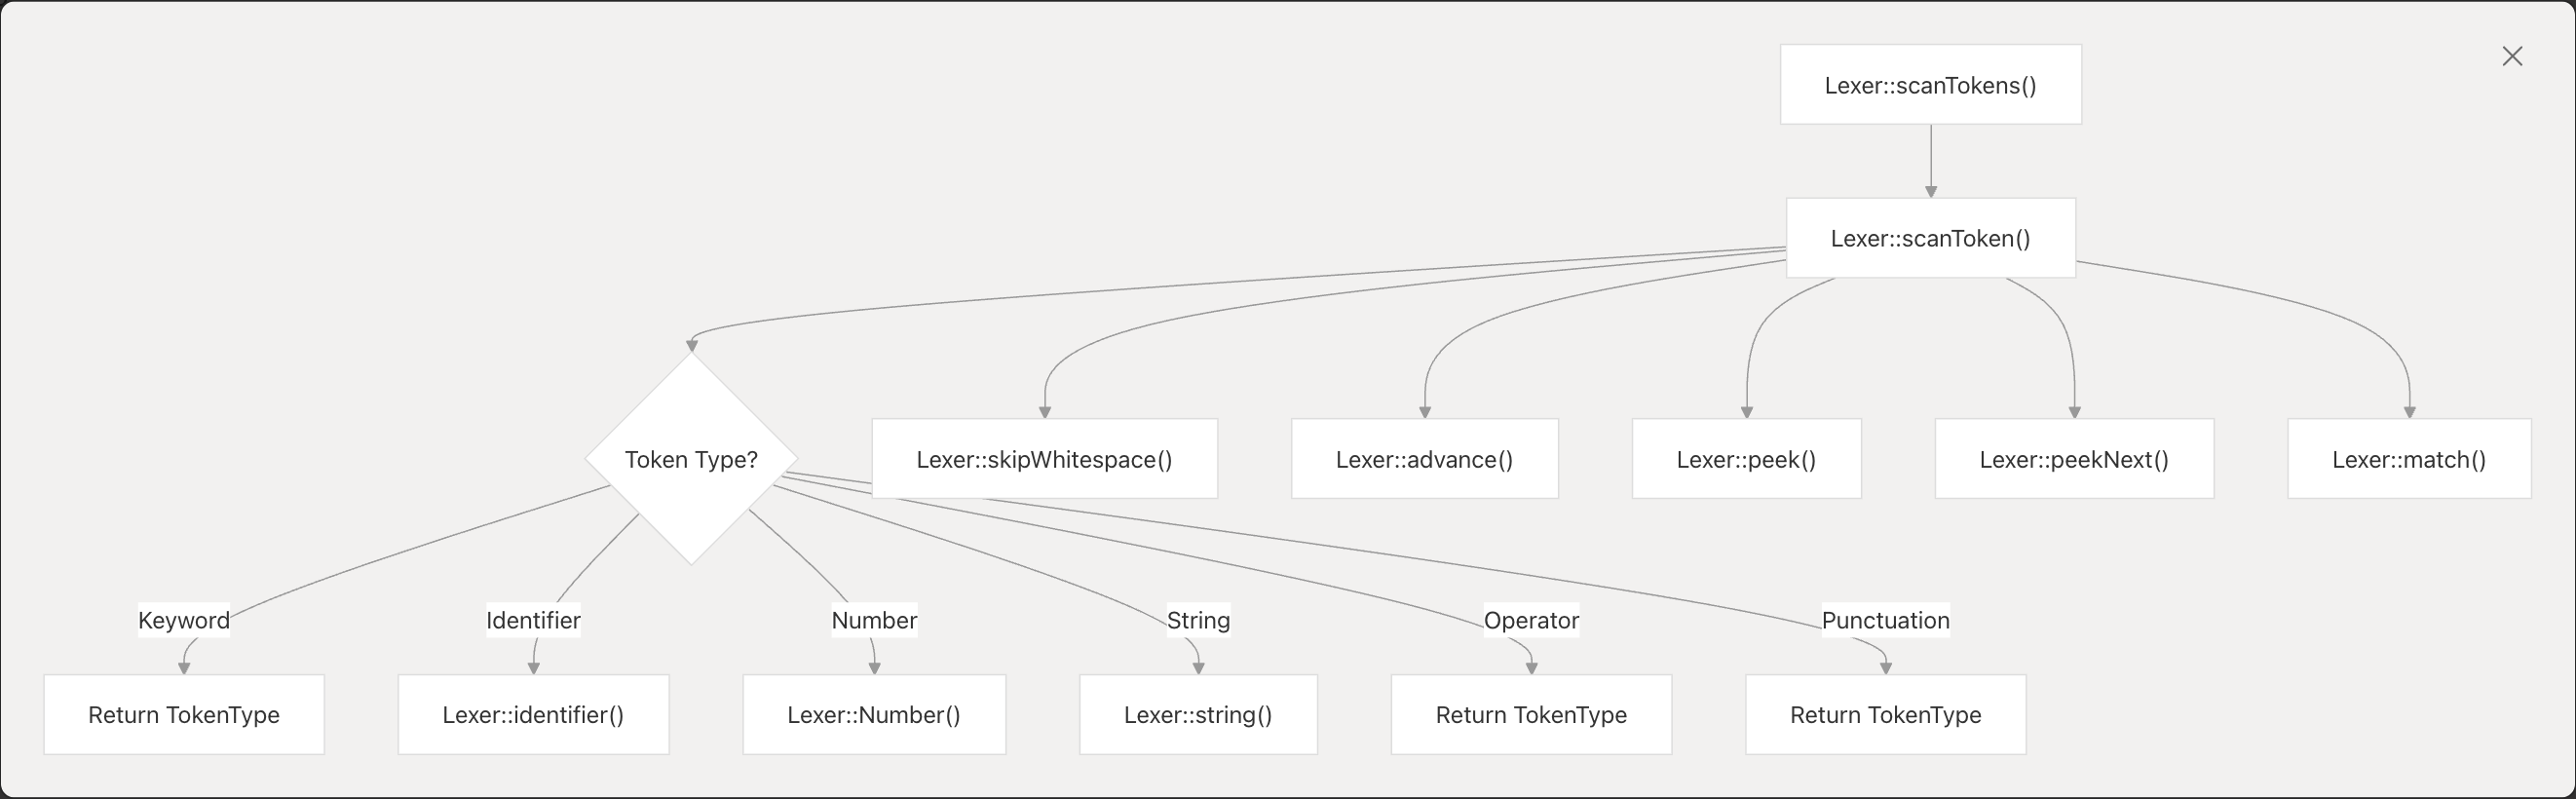
\includegraphics[width=1\linewidth]{lexer_imp.png}
        \caption{Lexer Implementation}
        \label{fig:enter-label}
    \end{figure}
The lexer employs a deterministic finite automaton (DFA) approach:
\begin{enumerate}
    \item Read input character by character.
    \item Maintain current state based on previous characters.
        \item Transition between states based on character class.
    \item When an accepting state is reached, emit the corresponding token.
    \item Handle error states with appropriate error messages.
\end{enumerate}

\subsection{Parser}
The parser constructs an Abstract Syntax Tree (AST) from the token stream, enforcing the syntactic rules of the Hanami language. This component is implemented in the \texttt{parser/} directory.
\begin{figure}[H]
    \centering
    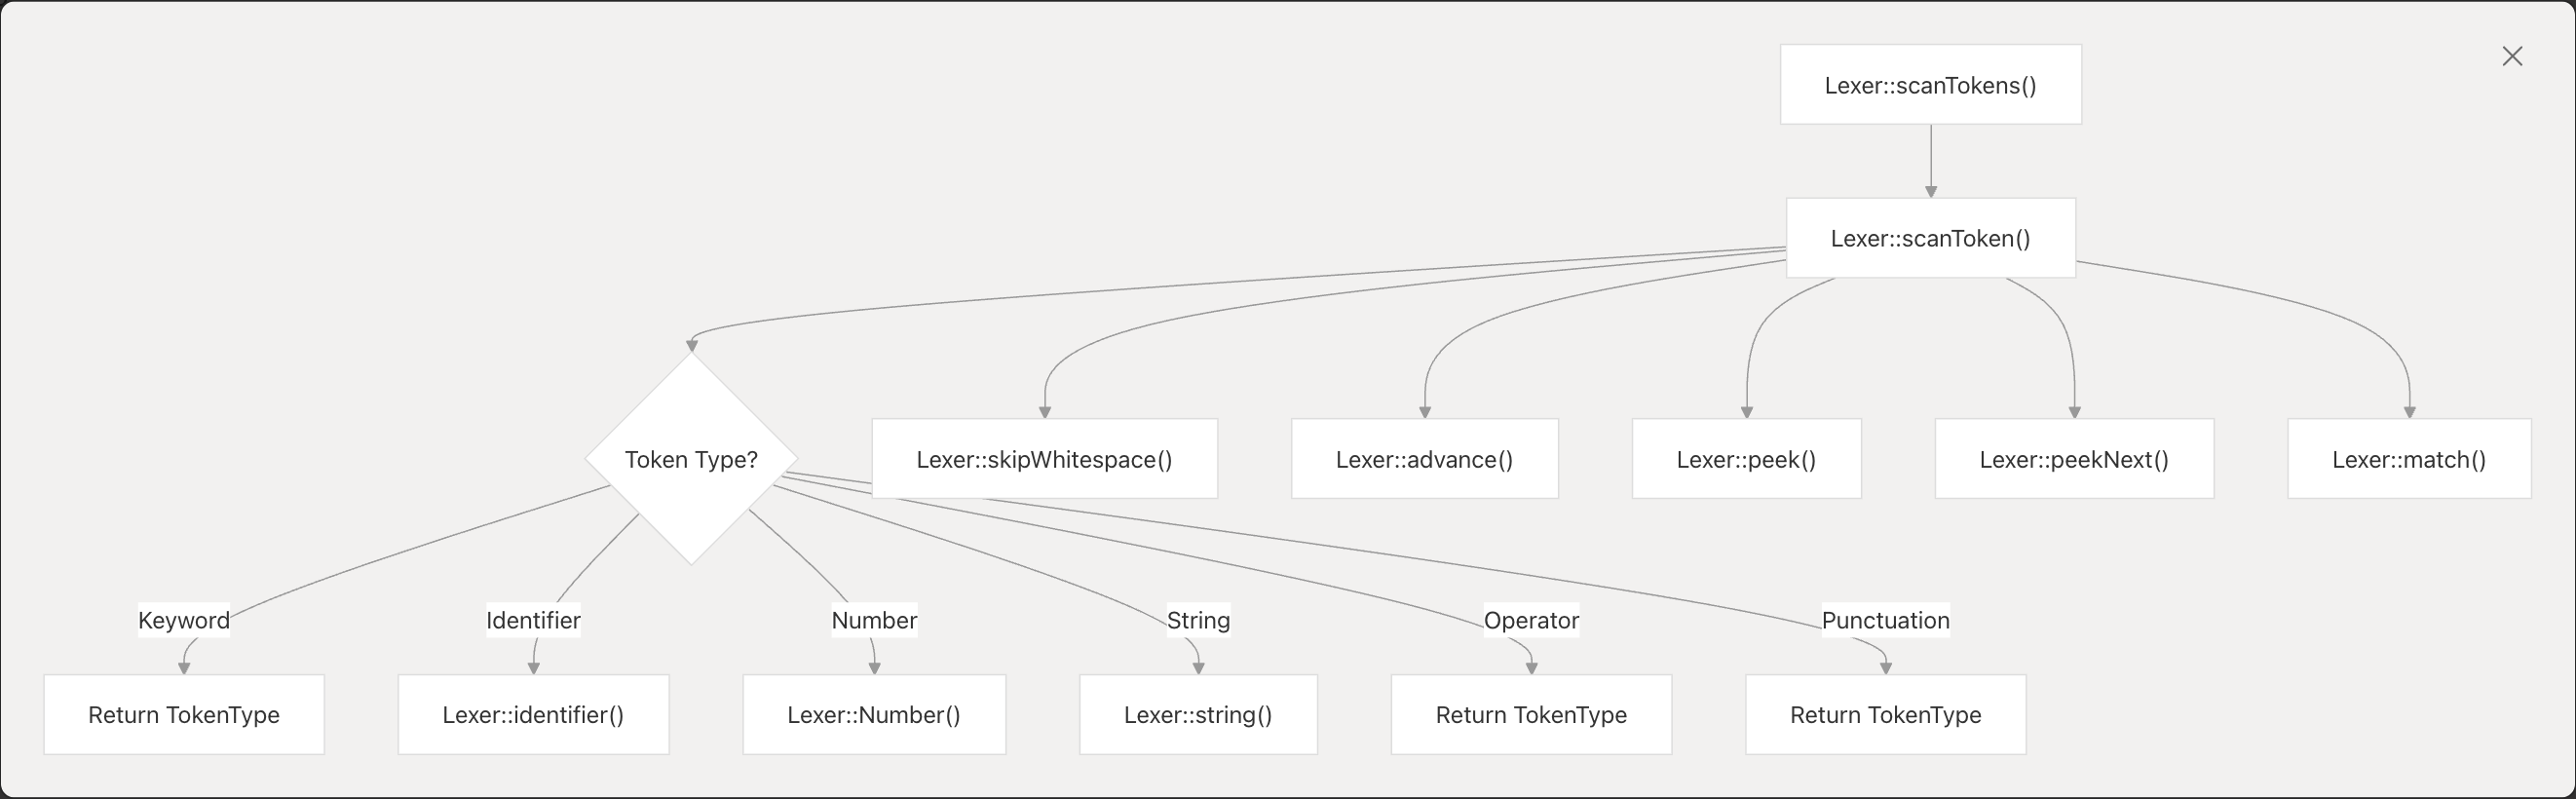
\includegraphics[width=1\linewidth]{lexer_imp}
    \caption{Parser Implementation}
    \label{fig:enter-label}
\end{figure}
\subsubsection{Parser Components}
\begin{itemize}
    \item \textbf{GrammarDefinition}: Formal definition of the Hanami language grammar.
    \item \textbf{Parser}: Implementation of parsing algorithms (recursive descent with predictive parsing).
    \item \textbf{ASTNodes}: Hierarchy of node types representing program constructs.
    \item \textbf{SyntaxErrorHandler}: Reports syntax errors with relevant context.
\end{itemize}

\subsubsection{Parsing Algorithm}
The parser uses a recursive descent approach with predictive parsing:
\begin{enumerate}
    \item Start with the top-level grammar rule.
    \item For each non-terminal in the rule, recursively apply its production rules.
    \item Match terminal symbols against the current token.
    \item Construct AST nodes as grammar rules are successfully matched.
    \item Handle synchronization points for error recovery.
\end{enumerate}

\subsubsection{AST Structure}
The AST is structured as a hierarchical composition of nodes representing different program constructs, including expressions, statements, declarations, and type specifications.

\subsection{Semantic Analyzer}
The semantic analyzer verifies the semantic correctness of the program and enriches the AST with type and scope information. This component is implemented in the \texttt{semantic\_analyzer/} directory.
\begin{figure}[H]
        \centering
        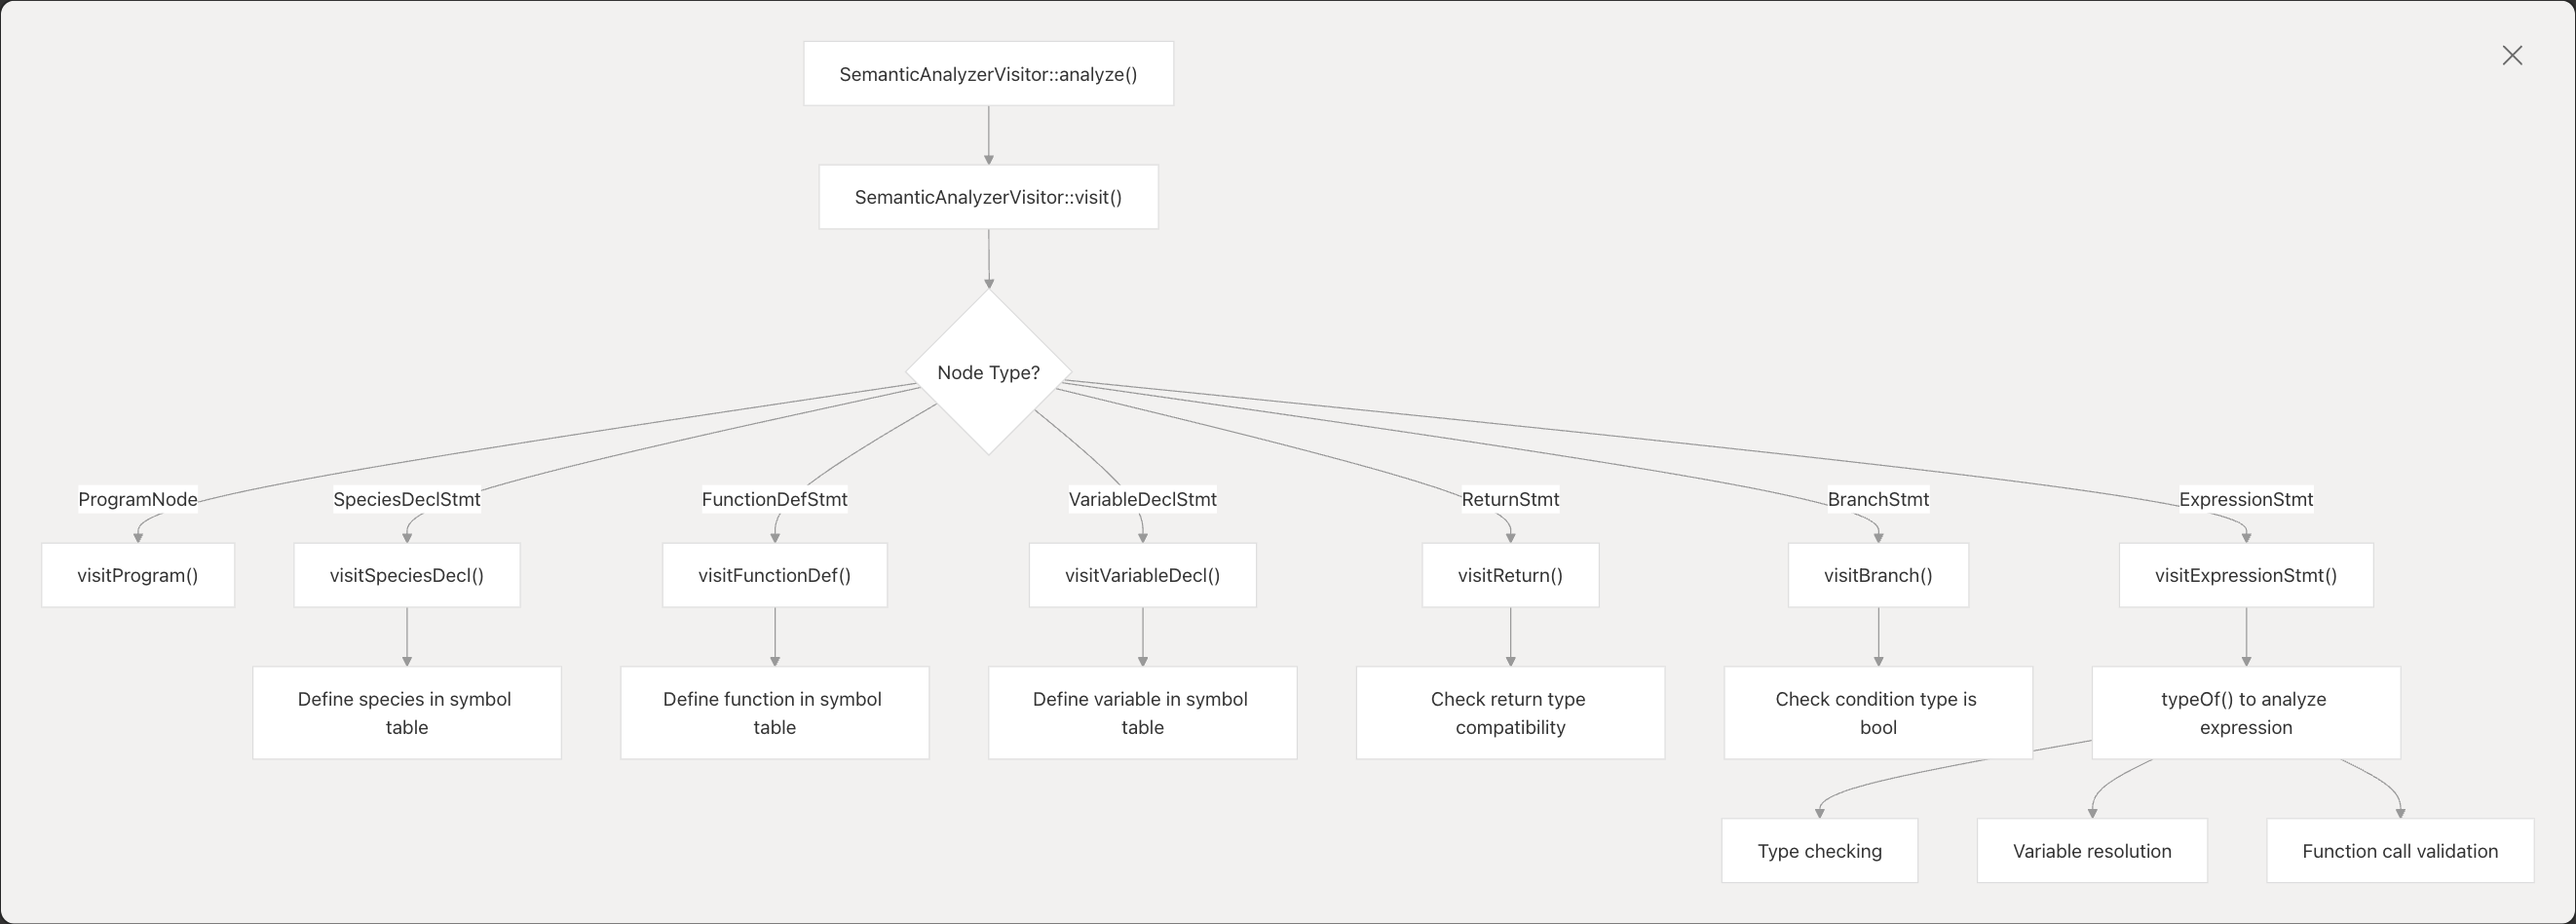
\includegraphics[width=1\linewidth]{seman_imp.png}
        \caption{Semantic Analyzer Implementation}
        \label{fig:enter-label}
    \end{figure}
\subsubsection{Semantic Analyzer Components}
\begin{itemize}
    \item \textbf{SymbolTable}: Manages symbols (variables, functions, types) and their attributes.
    \item \textbf{TypeSystem}: Defines and enforces the type rules of the Hanami language.
    \item \textbf{ScopeManager}: Tracks nested scopes and symbol visibility.
    \item \textbf{SemanticErrorReporter}: Reports semantic errors with contextual information.
\end{itemize}

\subsubsection{Symbol Table Structure}
The symbol table uses a hierarchical structure to represent nested scopes, allowing for efficient symbol lookup and scope management.

\subsubsection{Type System Details} % Renamed from "Type System" to avoid clash
The type system defines:
\begin{itemize}
    \item \textbf{Primitive Types}: int, float, bool, char, etc.
    \item \textbf{Compound Types}: arrays, structures, enums.
    \item \textbf{Type Relationships}: compatibility, conversion rules.
    \item \textbf{Type Checking}: assignment compatibility, operator operand verification.
\end{itemize}

\subsubsection{Semantic Analysis Process}
\begin{enumerate}
    \item Traverse the AST using the visitor pattern.
    \item Build and populate the symbol table.
    \item Perform type checking and inference.
    \item Validate semantic constraints (e.g., no duplicate declarations).
    \item Annotate the AST with semantic information.
\end{enumerate}

\subsection{Code Generator}
The code generator translates the semantically validated AST into target languages such as C++, Java, Python, or JavaScript. This component is implemented in the \texttt{codegen/} directory.
\begin{figure}[H]
    \centering
    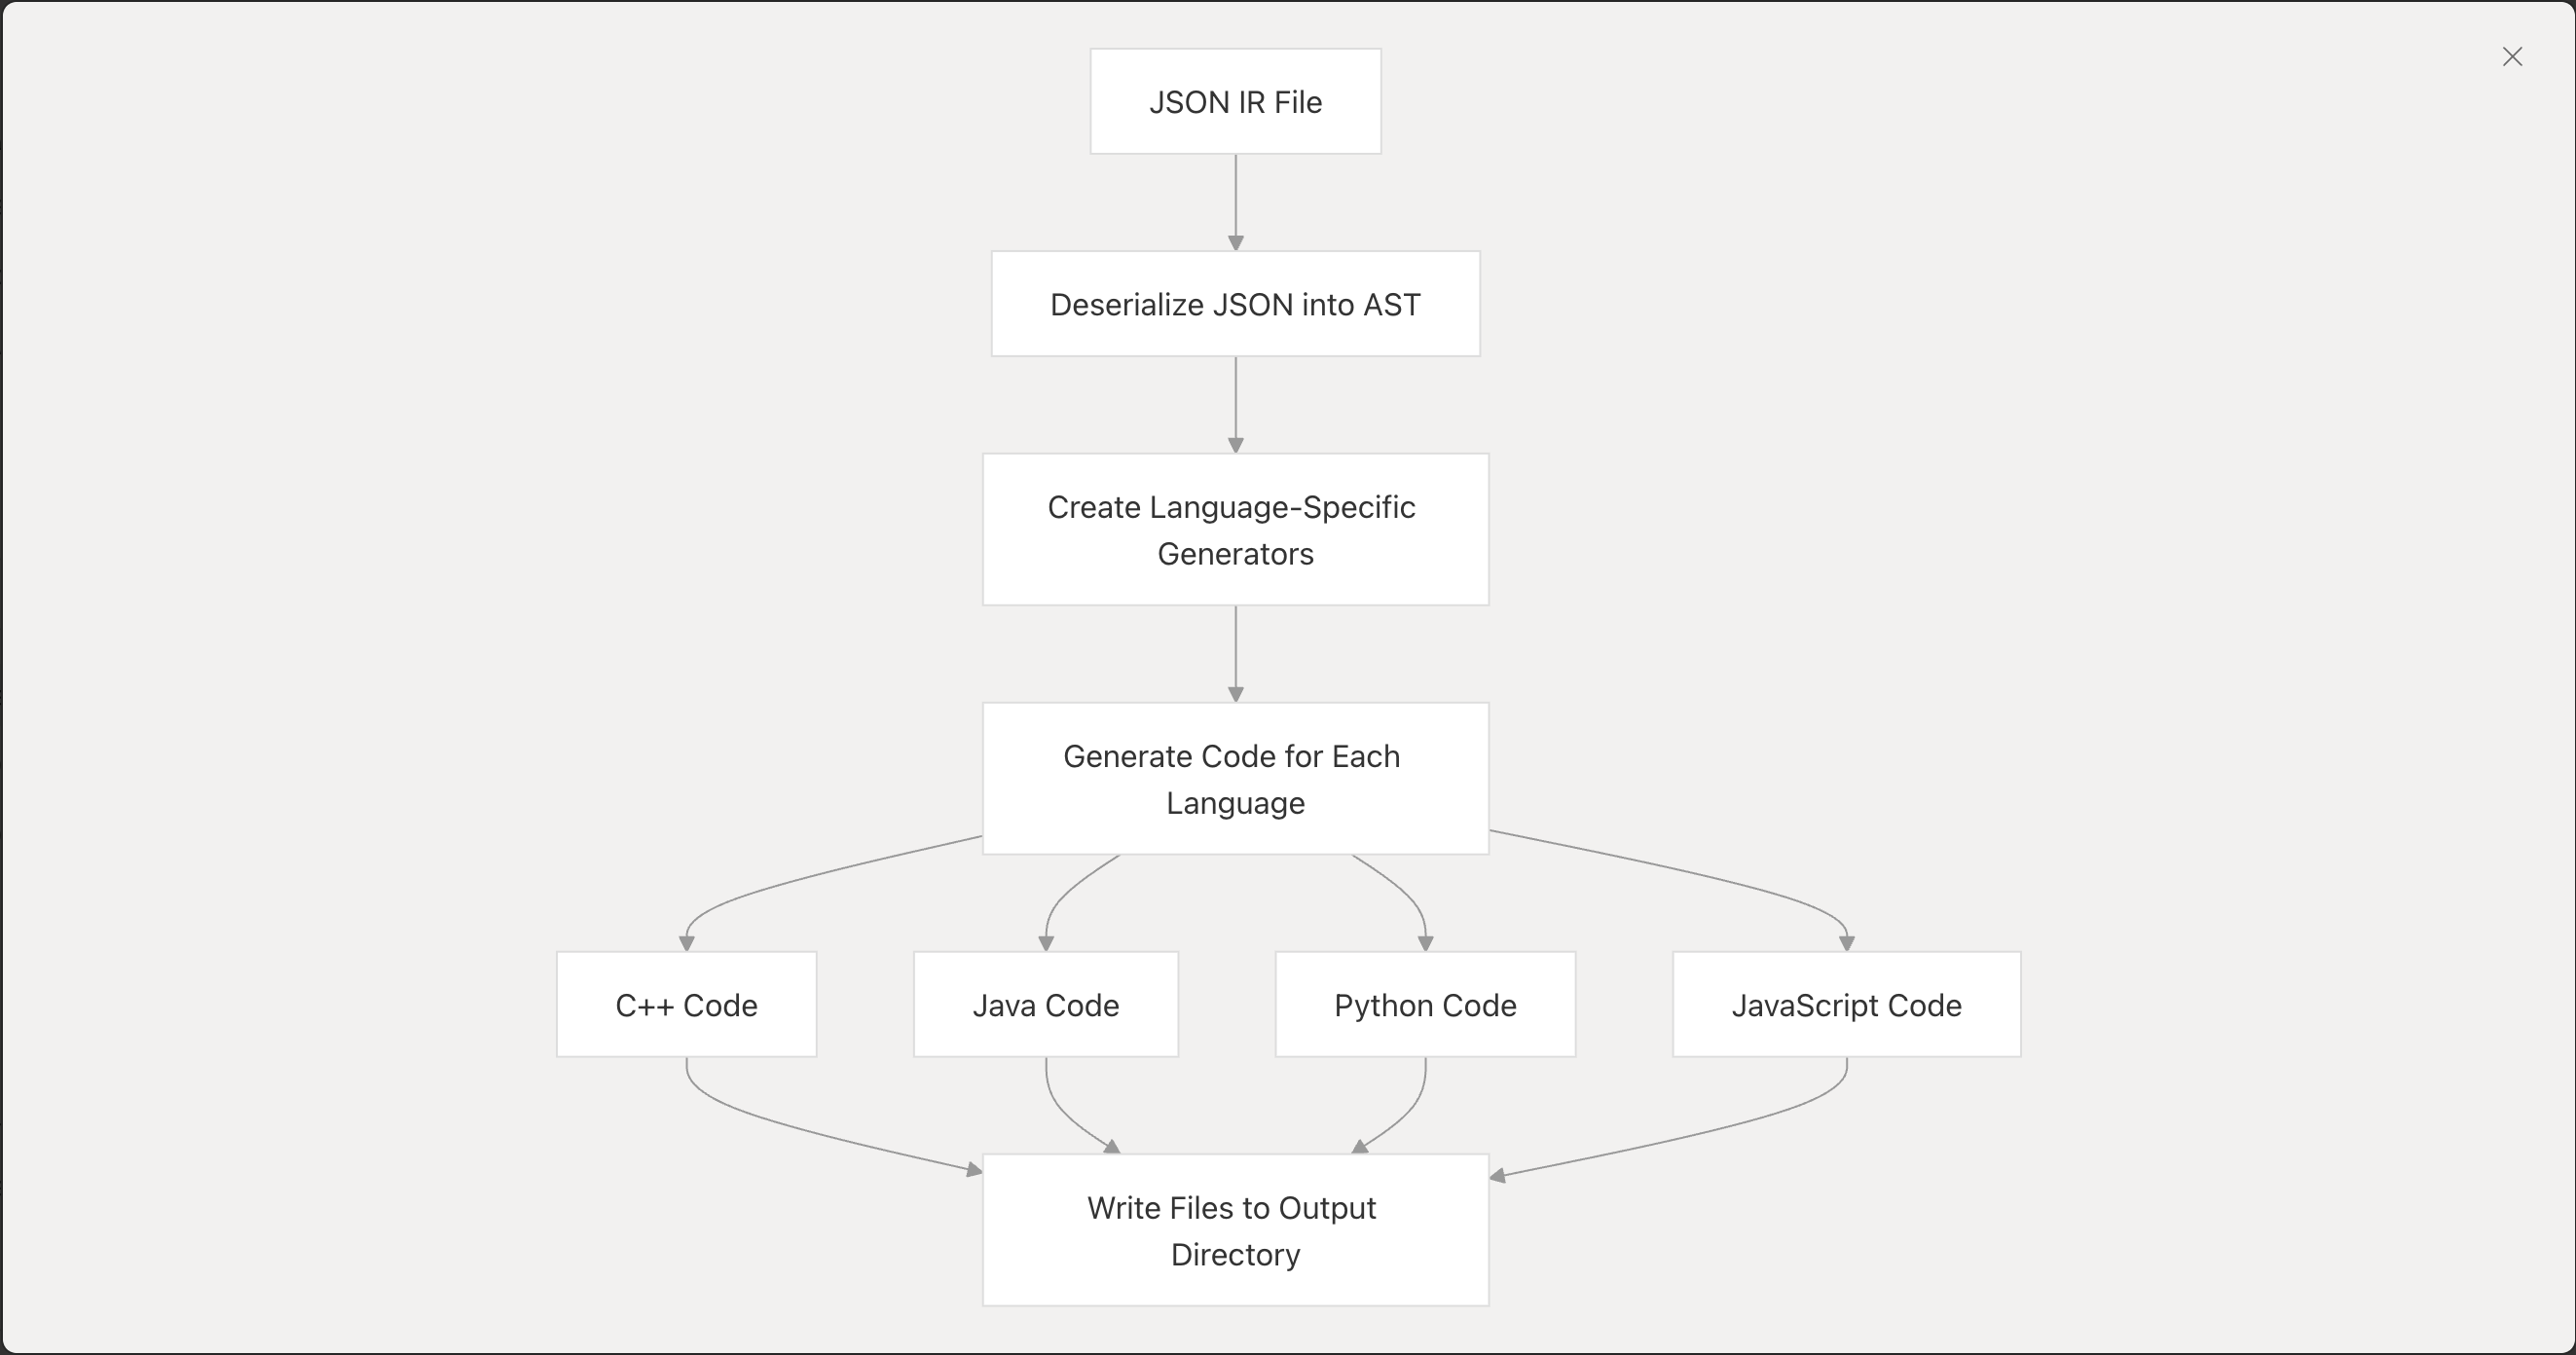
\includegraphics[width=1\linewidth]{codegen_flow.png}
    \caption{Code Generation Workflow}
    \label{fig:enter-label}
\end{figure}
\subsubsection{Code Generator Components}
\begin{itemize}
    \item \textbf{ASTVisitor}: Traverses the annotated AST.
    \item \textbf{CodeEmitter}: Generates code for the target language.
    \item \textbf{LanguageSpecificEmitter}: Handles specific syntax and semantics of the target language.
\end{itemize}

\subsubsection{Code Generation Process}
The code generation process involves:
\begin{itemize}
    \item Traverse the AST.
    \item Generate code for each node, considering the target language.
    \item Handle language-specific features and mappings. % Adjusted wording
    \item Output the generated code.
\end{itemize}

\subsubsection{Common Patterns in Code Generators}
All language-specific generators share similar structure and patterns:

\begin{itemize}
    \item Maintain a stringstream for accumulating generated code
    \item Track language-specific imports/includes
    \item Implement language-specific type mapping
    \item Implement language-specific operator mapping
    \item Handle language-specific syntax and semantics when visiting AST nodes
\end{itemize}

\subsubsection{Supported Target Languages} % Renamed from "Target Languages"
The code generator currently supports: % Adjusted wording
\begin{itemize}
    \item C++
    \item Java
    \item Python
    \item JavaScript % Added JS here too
\end{itemize}

\subsection{Support Systems}

\subsubsection{Build System}
The build system orchestrates the compilation process, managing dependencies and build configurations. It typically includes: % Adjusted wording
\begin{itemize}
    \item \textbf{Makefile/Build Script}: Defines build targets and dependencies.
    \item \textbf{Build Configuration}: Manages compiler flags and options.
    \item \textbf{Dependency Tracking}: Determines which files need recompilation.
\end{itemize}
Common build targets might include `clean`, `build`, `test`, `install`, and `package`. Build configurations often support Debug, Release, cross-compilation, and feature toggles.
\begin{figure}[H]
    \centering
    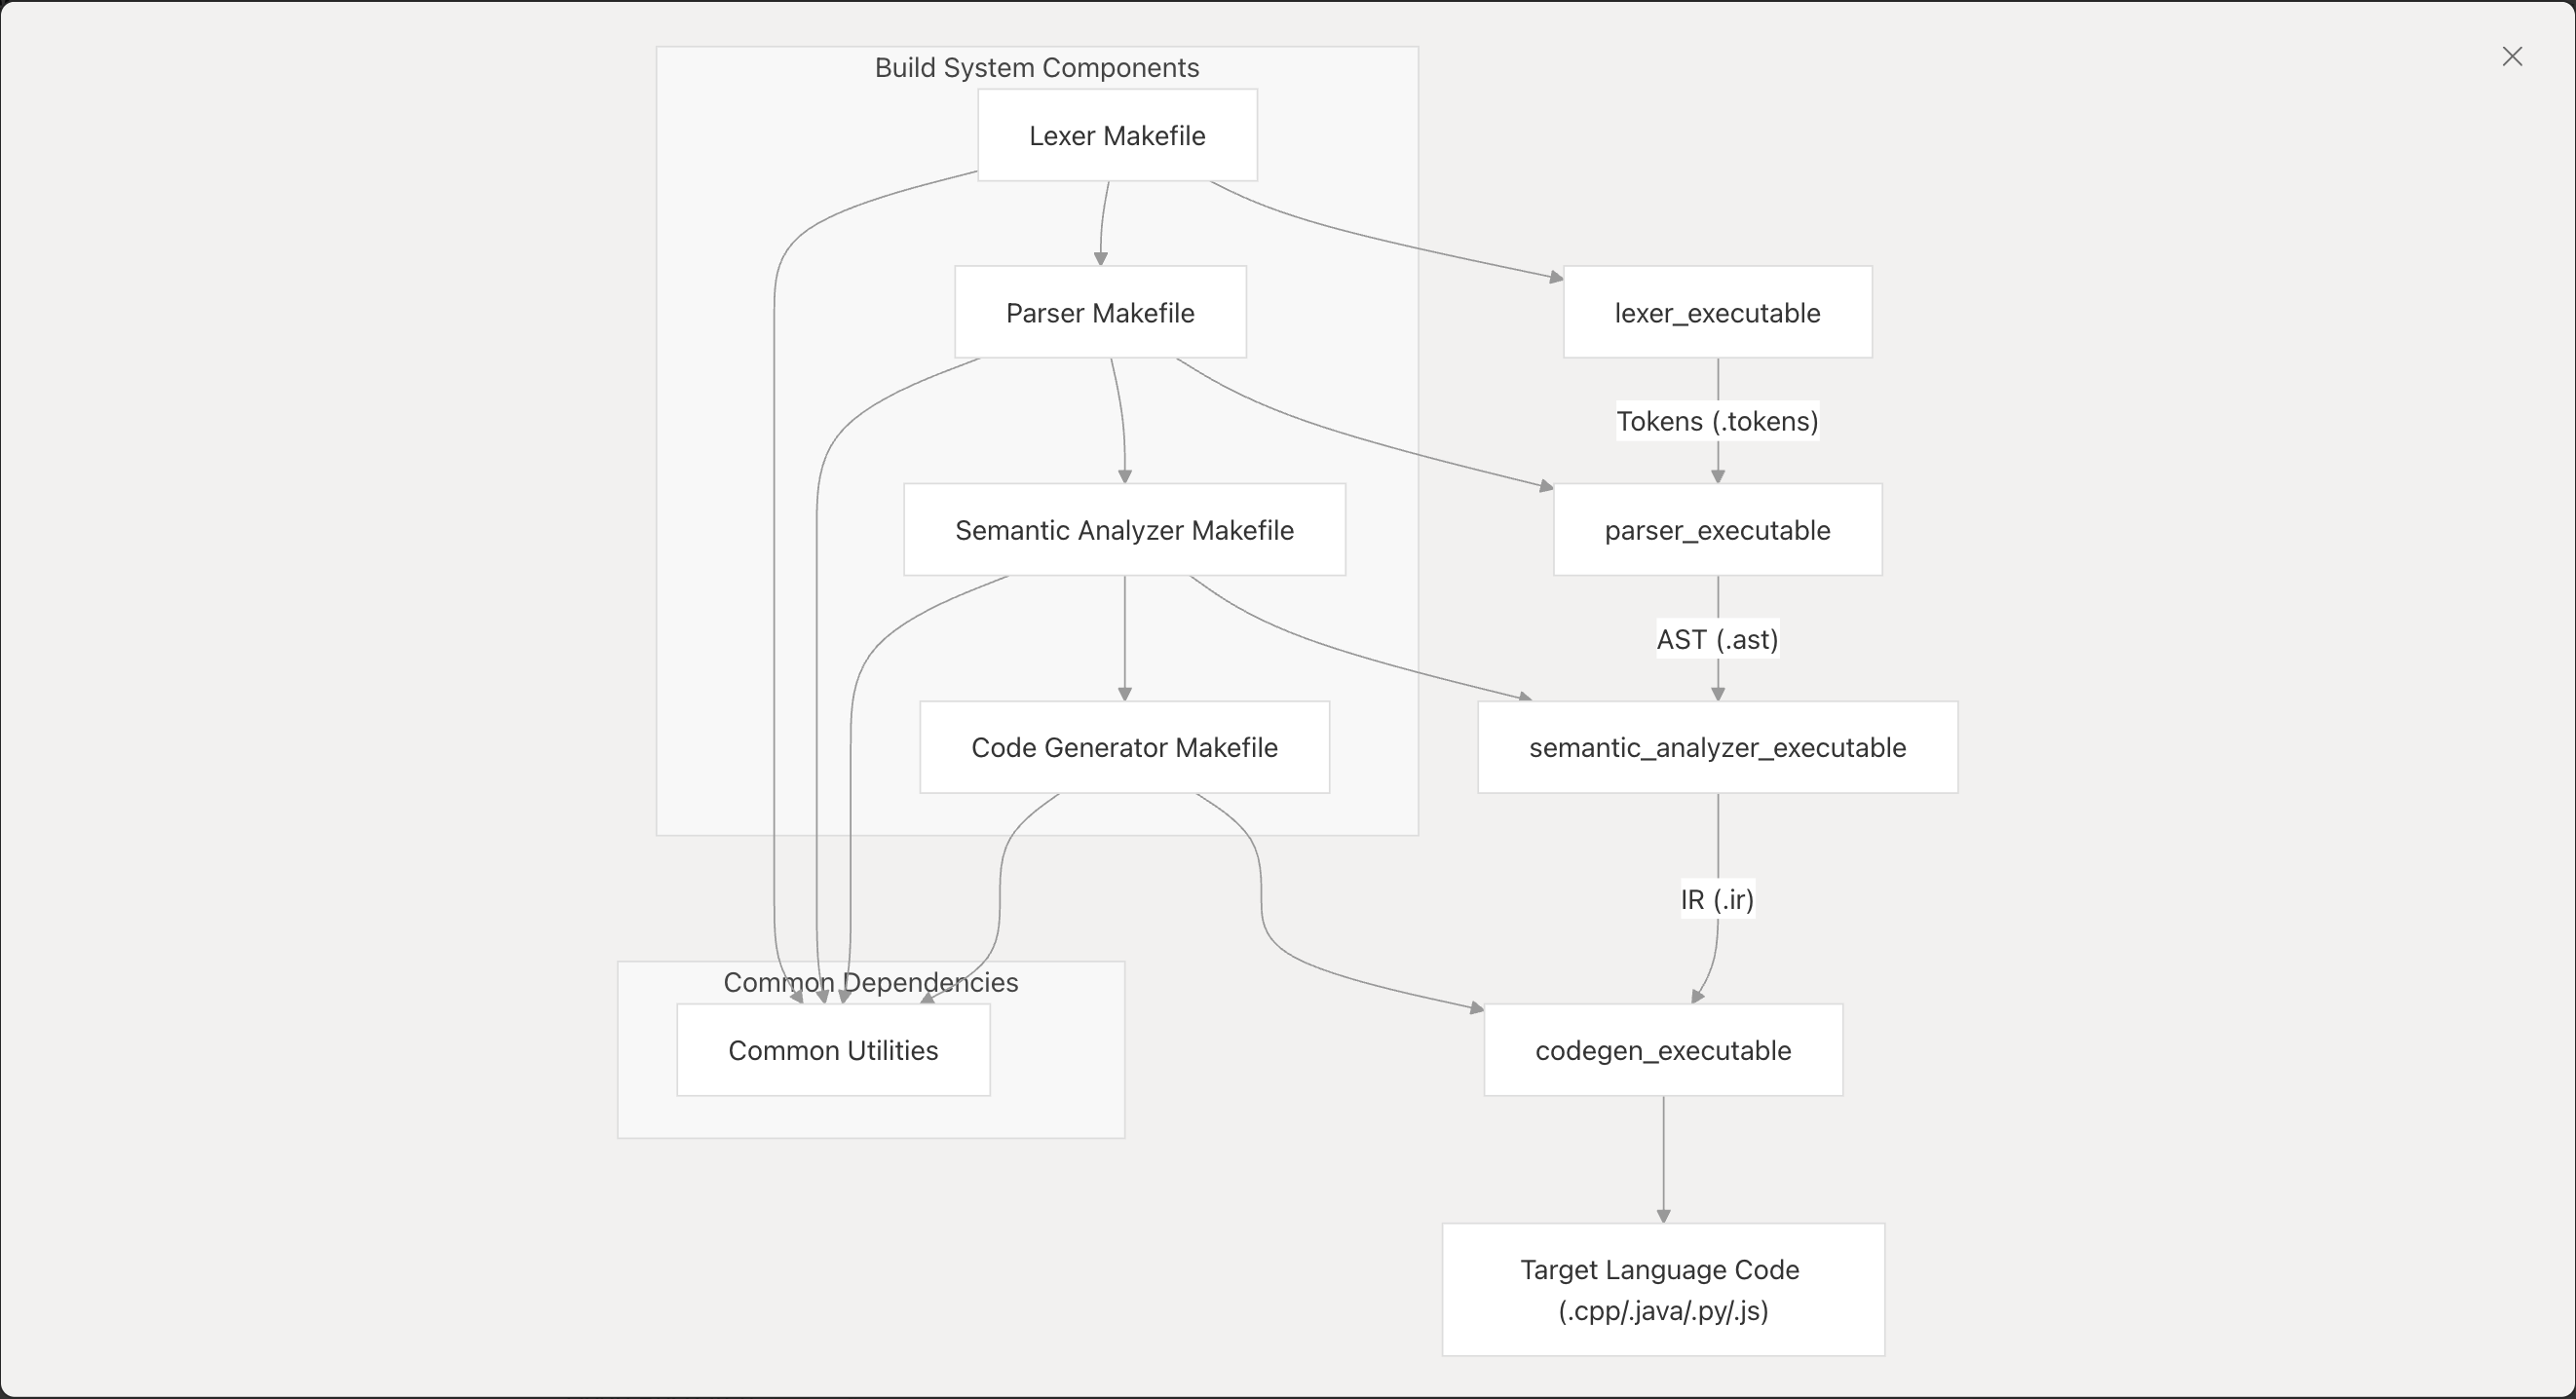
\includegraphics[width=1\linewidth]{buildsys.png}
    \caption{Build System Overview}
    \label{fig:enter-label}
\end{figure}

\textbf{Cross-Platform Support}:
The build system provides cross-platform support for both Windows and Unix-like operating systems:

Uses \$(OS) variable to detect Windows
Handles path differences between platforms
Adjusts deletion commands (del vs rm -f)
Handles output path formatting differences

\subsubsection{Common Utilities}
The \texttt{common/} directory contains shared utilities used across compiler components.
\begin{itemize}
    \item \textbf{Error Handling}: Consistent error reporting infrastructure.
    \item \textbf{Source Location Management}: Tracking file, line, and column information.
    \item \textbf{Memory Management}: Custom allocators or strategies. % Adjusted wording
    \item \textbf{Diagnostics}: Error and warning message formatting.
    \item \textbf{Data Structures}: Specialized structures like Symbol Tables, AST nodes, String Interning pools.
    \item \textbf{I/O Facilities}: For source reading, output generation, error streams.
\end{itemize}

\subsection{Inter-Component Communication}

\subsubsection{Data Exchange Formats}
Components communicate through well-defined data structures:
\begin{itemize}
    \item \textbf{Token Stream}: Between lexer and parser.
    \item \textbf{Abstract Syntax Tree (AST)}: Between parser and semantic analyzer.
    \item \textbf{Annotated AST}: Between semantic analyzer and code generator.
    \item \textbf{Target Language Code}: Output from code generator.
\end{itemize}

\subsubsection{Error Handling Strategy} % Renamed from "Error Handling"
The compiler implements a unified error handling strategy:
\begin{itemize}
    \item \textbf{Error Categories}: Lexical, syntactic, semantic, code generation.
    \item \textbf{Error Severity}: Fatal, error, warning, note.
    \item \textbf{Error Context}: Source location, relevant symbols, suggested fixes.
    \item \textbf{Error Recovery}: Mechanisms to continue compilation after errors where possible.
\end{itemize}

\subsubsection{Progress Tracking}
The compiler can track compilation progress for reporting: % Adjusted wording
\begin{itemize}
    \item Phase completion indications.
    \item Statistics (time, memory usage).
    \item Progress indicators for long operations.
\end{itemize}

\section{Evaluation}
\label{sec:evaluation}

During Hanami's development, we evaluated the language's functionality and the transpiler's correctness through several simple program examples. % Modified intro slightly

% --- Content integrated from system_architecture.tex (Section 9) ---

\subsection{Evaluation Approach}
Our evaluation focused on:
\begin{itemize}
    \item Basic algorithms (sorting, searching, string processing).
    \item Small programs demonstrating OOP (e.g., student management system, simple simulations).
    \item Basic file handling and I/O operations. % Combined from intro.tex list item
\end{itemize}
Testing involved writing Hanami code, transpiling it to each target language (C++, Java, Python, JavaScript), compiling/running the generated code, and verifying the output against expected results.

Although Hanami is not designed to compete with commercial programming languages, this evaluation provided valuable insights into factors affecting language usability and transpiler correctness.

\subsection{Performance Considerations}
The architecture was designed with performance considerations, though extensive optimization was outside the scope of this educational project:
\begin{itemize}
    \item \textbf{Modular Pipeline}: Allows potential parallelization of independent stages.
    \item \textbf{Memory Efficiency}: Use of appropriate data structures (e.g., AST, symbol tables).
    \item \textbf{Processing Time}: Algorithms chosen for reasonable performance (e.g., recursive descent parsing).
\end{itemize}
\subsubsection{Performance Results}

To evaluate the performance of the Garden language, we conducted an analysis of the execution time for each module during the compilation of two sample programs. The tests were designed to measure how the compiler performs with different types of programs.

\paragraph{Test Environment}
The evaluations were performed in the following environment:
\begin{itemize}
	\item IDE: Visual Studio Code v1.99.3
	\item CPU: Intel Core i7-11800H
	\item Measurement method: Using C++ \texttt{chrono} library
\end{itemize}

\paragraph{Sample Programs}
Two different programs were used for the evaluation:

\textbf{Program 1: Simple Calculator}
\begin{verbatim}
	style <iostream>
	
	garden SimpleProgram
	
	species SimpleCalculator {
		open:
		grow add(int a, int b) -> int {
			blossom a + b;
		}
		
		grow subtract(int a, int b) -> int {
			blossom a - b;
		}
		
		grow multiply(int a, int b) -> int {
			blossom a * b;
		}
		
		grow divide(int a, int b) -> int {
			branch (b == 0) {
				blossom 0;
			}
			blossom a / b;
		}
	};
	
	grow mainGarden() -> int {
		SimpleCalculator calc;
		
		// Print results directly instead of assigning to variables
		bloom << "Addition: " << calc.add(5, 3) << "\n";
		bloom << "Subtraction: " << calc.subtract(10, 4) << "\n";
		bloom << "Multiplication: " << calc.multiply(6, 7) << "\n";
		bloom << "Division: " << calc.divide(20, 5) << "\n";
		
		blossom 0;
	}
\end{verbatim}

\textbf{Program 2: Number Guessing Game}
\begin{verbatim}
	style <iostream>
	style <string>
	
	garden Main
	
	grow mainGarden() -> int 
	{
		std::string playerName;
		int guess;
		int secretNumber = 3;
		bool isCorrect;
		
		bloom << "Chao mung den voi tro choi doan so bi mat!" << "\n";
		bloom << "Vui long nhap ten cua ban: ";
		
		water >> playerName;
		
		bloom << "Xin chao, " << playerName << "!" << "\n";
		bloom << "Hay doan mot so tu 1 den 5." << "\n";
		bloom << "Nhap so ban doan: ";
		
		water >> guess;
		
		branch (guess < 1) 
		{
			bloom << "So ban nhap qua nho!" << "\n";
			bloom << playerName << ", so phai tu 1 den 5." << "\n";
			bloom << "Tro choi ket thuc." << "\n";
			blossom 0;
		}
		
		branch (guess > 5) 
		{
			bloom << "So ban nhap qua lon!" << "\n";
			bloom << playerName << ", so phai tu 1 den 5." << "\n";
			bloom << "Tro choi ket thuc." << "\n";
			blossom 0;
		}
		
		isCorrect = (guess == secretNumber);
		
		branch (isCorrect) 
		{
			bloom << "Chuc mung, " << playerName << "!" << "\n";
			bloom << "Ban da doan dung so bi mat: " << secretNumber << "\n";
			bloom << "Ban that xuat sac!" << "\n";
		}
		
		branch (isCorrect == false) 
		{
			bloom << "Rat tiec, " << playerName << "!" << "\n";
			bloom << "So ban doan khong dung." << "\n";
			bloom << "So bi mat la: " << secretNumber << "\n";
			bloom << "Hay thu lai lan sau nhe!" << "\n";
		}
		
		bloom << "Cam on ban da tham gia tro choi!" << "\n";
		
		blossom 0;
	}
\end{verbatim}

\paragraph{Compilation Performance Results}
The tables below present the execution time (in seconds) for each module during compilation of both programs:

\textbf{Program 1: Simple Calculator}
\begin{table}[h]
	\centering
	\begin{tabular}{|c|c|c|c|c|c|}
		\hline
		\textbf{Run} & \textbf{Lexer} & \textbf{Parser} & \textbf{Semantic Analyzer} & \textbf{Code Generator} & \textbf{Total} \\
		\hline
		1 & 0.300513 & 0.196235 & 0.00248 & 0.005205 & 0.504433 \\
		\hline
		2 & 0.269355 & 0.193547 & 0.001894 & 0.004807 & 0.469603 \\
		\hline
		3 & 0.267332 & 0.243762 & 0.001938 & 0.005553 & 0.518585 \\
		\hline
		4 & 0.339088 & 0.197705 & 0.001844 & 0.004578 & 0.543215 \\
		\hline
		5 & 0.268074 & 0.215145 & 0.001955 & 0.015425 & 0.500599 \\
		\hline
		\textbf{Average} & 0.288872 & 0.209279 & 0.002022 & 0.007114 & 0.507287 \\
		\hline
	\end{tabular}
	\caption{Execution times (seconds) for Simple Calculator program}
	\label{tab:performance_results_prog1}
\end{table}

\textbf{Program 2: Number Guessing Game}
\begin{table}[h]
	\centering
	\begin{tabular}{|c|c|c|c|c|c|}
		\hline
		\textbf{Run} & \textbf{Lexer} & \textbf{Parser} & \textbf{Semantic Analyzer} & \textbf{Code Generator} & \textbf{Total} \\
		\hline
		1 & 0.39105 & 0.31098 & 0.00212 & 0.005749 & 0.709899 \\
		\hline
		2 & 0.42322 & 0.33467 & 0.00267 & 0.197931 & 0.958491 \\
		\hline
		3 & 0.425052 & 0.335004 & 0.00252 & 0.006645 & 0.769221 \\
		\hline
		4 & 0.410657 & 0.32318 & 0.002525 & 0.01027 & 0.746632 \\
		\hline
		5 & 0.446285 & 0.292156 & 0.002157 & 0.006017 & 0.746615 \\
		\hline
		\textbf{Average} & 0.419253 & 0.319198 & 0.002398 & 0.045322 & 0.786172 \\
		\hline
	\end{tabular}
	\caption{Execution times (seconds) for Number Guessing Game program}
	\label{tab:performance_results_prog2}
\end{table}

\paragraph{Comparative Analysis}
Comparing the performance metrics between the two programs:

\begin{itemize}
	\item \textbf{Overall Performance}: Program 2 (Number Guessing Game) took approximately 55\% longer to compile than Program 1 (Simple Calculator), with average total times of 0.786s vs. 0.507s.
	
	\item \textbf{Lexer}: The lexical analysis for Program 2 took 45\% longer (0.419s vs. 0.289s), which correlates with its larger size and more complex structure.
	
	\item \textbf{Parser}: The parsing phase for Program 2 required about 53\% more time (0.319s vs. 0.209s), reflecting the increased complexity of the control flow with multiple branch statements.
	
	\item \textbf{Semantic Analyzer}: The semantic analysis showed only a minimal increase (0.0024s vs. 0.0020s), suggesting that this phase scales well with program complexity.
	
	\item \textbf{Code Generator}: The most significant difference was in the code generation phase, where Program 2 required approximately 6.4 times longer (0.045s vs. 0.007s). This is largely due to the second run's anomalous value of 0.198s, which may indicate occasional optimization challenges or resource contention.
\end{itemize}

\paragraph{Conclusions}
The performance analysis reveals that:

\begin{itemize}
	\item The Lexer and Parser continue to be the most time-consuming phases of the compilation process for both programs, accounting for over 90\% of the total time.
	
	\item The compilation time increases with program complexity and size, but not linearly across all phases.
	
	\item The Semantic Analyzer demonstrates excellent scalability, with minimal performance impact as program complexity increases.
	
	\item The Code Generator shows more variability in performance, suggesting it may benefit from further optimization to handle more complex programs consistently.
	
	\item For both programs, the total compilation time remains under one second, which is acceptable for development purposes, though further optimizations could improve the developer experience for larger codebases.
\end{itemize}


\subsection{Scalability Aspects}
The architecture supports language and compiler evolution:
\begin{itemize}
    \item \textbf{Feature Extensibility}: Clear separation of concerns facilitates adding new language features.
    \item \textbf{Target Platform Addition}: The code generator's visitor pattern makes adding new target languages relatively modular.
    \item \textbf{Optimization Expansion}: A framework for adding intermediate representations or optimization passes could be integrated later.
\end{itemize}

\subsection{Maintainability Factors}
The architecture promotes maintainability:
\begin{itemize}
    \item \textbf{Component Isolation}: Minimizing inter-component dependencies simplifies updates.
    \item \textbf{Interface Stability}: Clear data structures (Tokens, AST) serve as contracts between phases.
    \item \textbf{Testing Support}: Modular design facilitates unit testing of individual components.
\end{itemize}

\subsection{Quality Assurance}
The architecture includes provisions for quality assurance:
\begin{itemize}
    \item \textbf{Verification Points}: Semantic analysis acts as a key validation step.
    \item \textbf{Diagnostic Capabilities}: Emphasis on clear error reporting with source locations.
    \item \textbf{Tracing Infrastructure}: Potential for adding logging or debugging outputs throughout the pipeline.
\end{itemize}


% --- Content from introduction.tex (Limitations and Future Work) ---
\subsection{Limitations}
As a student project, Hanami has several limitations that could be addressed in future work:
\subsubsection{Lack of Basic Data Structures}
The current version of Hanami lacks support for several essential data structures:
\begin{itemize}
\item \textbf{No array declaration syntax} - Cannot store and manipulate collections of data
\item \textbf{Lack of element access operators} - Cannot access elements in data structures
\item \textbf{No support for collections} - Limited ability to process sets and relational data
\end{itemize}
A desired implementation would include:
\begin{verbatim}
// Array declaration
int numbers[5];
int initialized[] = {1, 2, 3, 4, 5};
// Array access
numbers[0] = 10;
bloom << numbers[2];
\end{verbatim}
\subsubsection{Limitations in String Handling}
Hanami lacks comprehensive string manipulation features:
\begin{itemize}
\item No string interpolation
\item Limited string operations
\item No regular expression support
\end{itemize}
\subsubsection{Limited Control Structures}
\paragraph{Switch/Case Statements}
Hanami currently lacks a switch/case construct, which is essential for multi-path branching logic:
\begin{verbatim}
switch (value) {
case 1:
bloom << "One";
break;
case 2:
bloom << "Two";
break;
default:
bloom << "Other";
}
\end{verbatim}
\paragraph{Advanced Flow Control}
The language lacks several modern flow control constructs:
\begin{itemize}
\item Exception handling mechanisms
\item Iterators and enhanced for-loops
\item Pattern matching
\item Asynchronous programming constructs
\end{itemize}
\subsubsection{Language Feature Limitations}
\paragraph{Object-Oriented Programming Limitations}
The current implementation has several OOP limitations:
\begin{itemize}
\item \textbf{Incomplete inheritance model} - Lacks multiple inheritance and interface implementation
\item \textbf{No polymorphism} - Unable to use dynamic dispatch effectively
\item \textbf{Limited access control} - Insufficient granularity in member visibility
\end{itemize}
\paragraph{Functional Programming Limitations}
Hanami lacks modern functional programming features:
\begin{itemize}
\item No lambda expressions or first-class functions
\item No higher-order functions
\item No function composition utilities
\end{itemize}

These limitations also present learning opportunities for future iterations or subsequent projects in the CS3370 class.

\subsection{Future works}
\subsubsection{Enhancing Language Syntax}
\paragraph{Data Structure Improvements}
To address the current lack of fundamental data structures, we will implement:
\begin{itemize}
\item \textbf{Comprehensive array system} with intuitive syntax for declaration, initialization, and access
\item \textbf{Built-in collection types} including lists, sets, maps, and queues with optimized performance
\item \textbf{Advanced data structure operations} including slicing, filtering, and mapping
\end{itemize}
Example of planned array implementation:
\begin{verbatim}
// Flexible array declaration and initialization
arr[int] numbers = [1, 2, 3, 4, 5];
arr[string] names = ["Alice", "Bob", "Charlie"];
// Advanced operations
numbers[1..3] = [10, 20];  // Slice assignment
var doubled = numbers.map(n => n * 2);  // Transformation
\end{verbatim}
\paragraph{String Handling Enhancement}
We will implement advanced string handling capabilities:
\begin{itemize}
\item \textbf{String interpolation} with embedded expressions
\item \textbf{Built-in regular expression support} with intuitive syntax
\item \textbf{Extensive string manipulation functions} for common operations
\end{itemize}
Example of planned string features:
\begin{verbatim}
// String interpolation
var name = "World";
var greeting = "Hello ${name}!";  // "Hello World!"
// Regular expressions
var isEmail = "user@example.com" ~= /^[\w.]+@[\w.]+.\w+$/;
\end{verbatim}
\subsubsection{Control Structure Enhancements}
\paragraph{Pattern Matching}
We will implement a powerful pattern matching system that goes beyond traditional switch/case:
\begin{verbatim}
match (value) {
case int n if n > 0 => bloom << "Positive number: ${n}";
case int n if n < 0 => bloom << "Negative number: ${n}";
case string s => bloom << "String: ${s}";
case Person(name: var n, age: var a) =>
bloom << "Person ${n}, age ${a}";
case [var head, *var tail] =>
bloom << "List with head ${head}";
case _ => bloom << "Default case";
}
\end{verbatim}
\paragraph{Exception Handling}
A robust exception handling system will be implemented:
\begin{verbatim}
try {
// Code that might throw exceptions
var result = riskyOperation();
} catch (FileNotFound e) {
// Handle specific exception
bloom << "File not found: ${e.message}";
} catch (e: NetworkError | TimeoutError) {
// Handle multiple exception types
bloom << "Connection issue: ${e.message}";
} finally {
// Always executed
cleanup();
}
\end{verbatim}
\subsubsection{Unique Features and Advantages}
\paragraph{Bidirectional Type Inference}
Unlike many languages with limited type inference, Hanami will feature bidirectional type inference that provides both safety and conciseness:
\begin{itemize}
\item \textbf{Local and global inference} that reduces type annotations while maintaining type safety
\item \textbf{Partial type annotations} allowing developers to specify only critical types
\item \textbf{Flow-sensitive typing} that understands type changes through control flow
\end{itemize}
\begin{verbatim}
// Type inferred from initialization
var x = 5;  // inferred as int
var y = "hello";  // inferred as string
// Flow-sensitive typing
var z = getValueFromNetwork();
if (z is int) {
// z is treated as int in this scope
bloom << z + 10;
}
\end{verbatim}
\subsubsection{Context-Aware Compilation}
Hanami will introduce a revolutionary context-aware compilation system:
\begin{itemize}
\item \textbf{Adaptive optimization} based on usage patterns
\item \textbf{Contextual code suggestions} during development
\item \textbf{Runtime performance profiling} that feeds back into the compiler
\end{itemize}
This system will allow Hanami to optimize code based on how it's actually used rather than generic optimization strategies.

\section{Conclusion} % Placeholder for conclusion
\label{sec:conclusion}

% Add concluding remarks here. Summarize the project, reiterate its educational value, and perhaps briefly touch on the key findings or future directions.
This paper presented Hanami, a programming language developed as an educational project within the CS3370 course. By designing and implementing a transpiler targeting multiple languages (C++, Java, Python, JavaScript), we gained hands-on experience with lexical analysis, parsing, semantic analysis, and code generation. The nature-inspired syntax and features like multi-target transpilation served as practical vehicles for exploring language design principles and trade-offs. The modular architecture proved effective for managing complexity and demonstrated key software engineering concepts relevant to compiler construction. While limitations exist, the Hanami project successfully met its educational objectives, providing a tangible framework for applying theoretical programming language concepts and fostering a deeper understanding of compiler design.


% Bibliography Inclusion (Choose one method)

% Method 1: Use the pre-compiled .bbl file (as in original introduction.tex)
% Ensure 'document.bbl' exists in the same directory or provide the correct path.
% \input{document.bbl} % Commented out for now, uncomment if needed

% Method 2: Use BibTeX with a .bib file
% Replace 'references' with the actual name of your .bib file (without the .bib extension)
\bibliographystyle{IEEEtran}
\bibliography{references} % Assuming you have a references.bib file
\newpage
\section{Appendix}
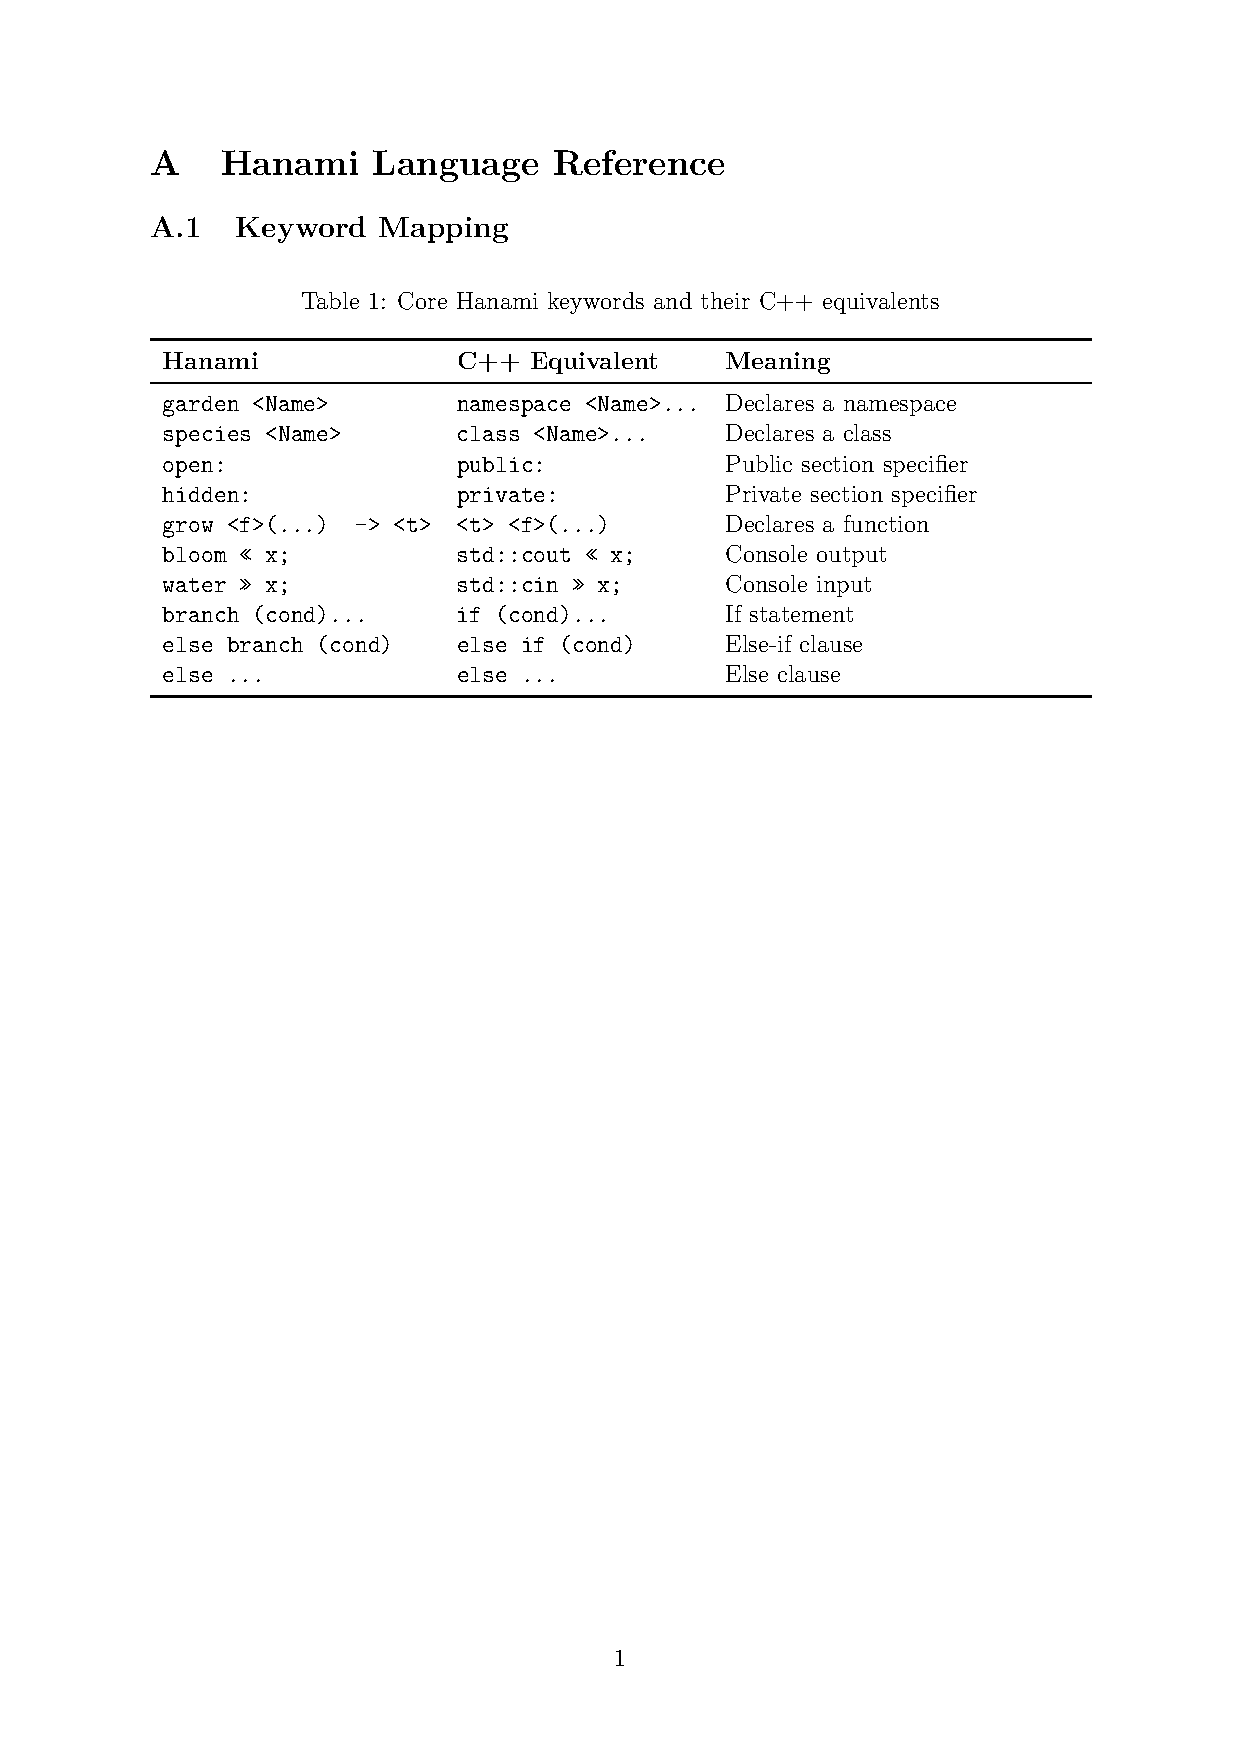
\includepdf[pages=-]{appendix.pdf} % Include all pages from appendix.pdf


\end{document}